\documentclass[11pt,a4paper]{article}

% These are extra packages that you might need for writing the equations:
\usepackage{amsmath}
\usepackage{amsfonts}
\usepackage{amssymb}
\usepackage{physics}
\usepackage{url}
\usepackage{graphicx}
\usepackage[left=2cm,right=2cm,top=2cm,bottom=2cm]{geometry}
\usepackage[section]{placeins}
\usepackage{gensymb}
\usepackage[section]{placeins}
\usepackage{siunitx}
\usepackage{slashed}
\usepackage{tikz-feynman}

\begin{document}

% Enter the exercise number, your name and date here:
\begin{titlepage}
	\begin{center}

		\vspace*{0cm}

		
\includegraphics[width=0.4\textwidth]{fig/uzh.png}

		\vspace*{5cm}

		\Huge
		\textbf{Top quark pair production and W boson charge asymmetry}
				
		\vspace{1.5cm}
		\LARGE
		EPP report, June 2021
				
		\vspace{1.5cm}
				
		\textbf{Luca Naterop}
				
		\vfill				

		\vfill
				
		\Large

					
	\end{center}
\end{titlepage}

\section{Introduction}
Top quarks, initially observed at the Fermilab Tevatron collider \cite{ttbarobs}, can be produced at $\sqrt{s} = 7$ TeV at the LHC \cite{lhc}. Almost always, they decay via the electroweak interactions to $W$ bosons and $b$ quarks. Such an event can be pictured as
\begin{equation}
	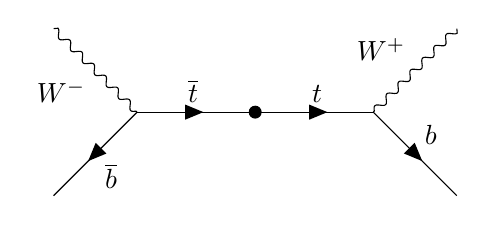
\begin{tikzpicture}
		\begin{feynman}
			\node[dot] (c);
			\vertex [right= of c] (t1);
			\vertex [left= of c] (t2);
			\vertex [above right= of t1] (W1);
			\vertex [below right= of t1] (b1);
			\vertex [above left= of t2] (W2);
			\vertex [below left= of t2] (b2);
			\diagram*{
				(c) [dot] --[fermion, edge label = \(t\)] (t1),
				(t2) --[fermion, edge label = \(\overline{t}\)] (c),
				(t1) --[photon, edge label = \(W^+\)] (W1),
				(t1) --[fermion, edge label = \(b\)] (b1),
				(t2) --[photon, edge label = \(W^-\)] (W2),
				(t2) --[fermion, edge label = \(\overline{b}\)] (b2),<
			};
		\end{feynman}
	\end{tikzpicture}
\end{equation}
where the $W$ bosons can decay to $q \overline{q}$ or to a lepton and a neutrino. In this report, we analyze 50 $pb^{-1}$ data recorded from the Compact Muon Solenoid (CMS) experiment in order to measure the $t \overline{t}$ cross section in the semileptonic (muon) channel, which is done in section 2. In section 3, we measure the $W$ boson charge asymmetry as a function of the isolated muon rapidity. 
\\
\\
The full python3 code that was used to produce the results in this report is located in the github repository at \url{https://github.com/lucnat/epp-project}.
\section{Top production cross section}
\subsection{Event selection and signal reconstruction}
In order to estimate a cross section from the data, the first step is to discriminate events which stem from the process of interest
\begin{equation}
	t \, \overline{t} \; \rightarrow \; \mu \, \nu \, b \, \overline{b} \, q \, \overline{q} 
\end{equation}
from background events, which consists of events with a similar signature. To achieve this, we use tagged Monte-Carlo (MC) data and plot these as a function of a number of discriminator variables, on which cuts are applied. In the present case, an event is treated as a signal event if there is exactly one isolated muon with transverse momentum $p_T > 25$ GeV, where an isolated muon is one for which the relative isolation $I_\text{muon} / p_T < 0.03$. Additionally, in order to eliminate Drell-Yan background, we ask for at least four hadronic jets, of which at least one must have $p_T > 25$ GeV and at least one must be B-tagged. This still leaves a considerable amount of QCD background, most of which is eliminated by also requiring a minimum missing transverse energy of $\slashed{E} > 20$ GeV. Finally, events are required to be triggered using the variable triggerIsoMu24. 
\begin{figure}[!htb]
	\begin{center}
		\begin{tikzpicture}
			\node[inner sep=0pt] (A) {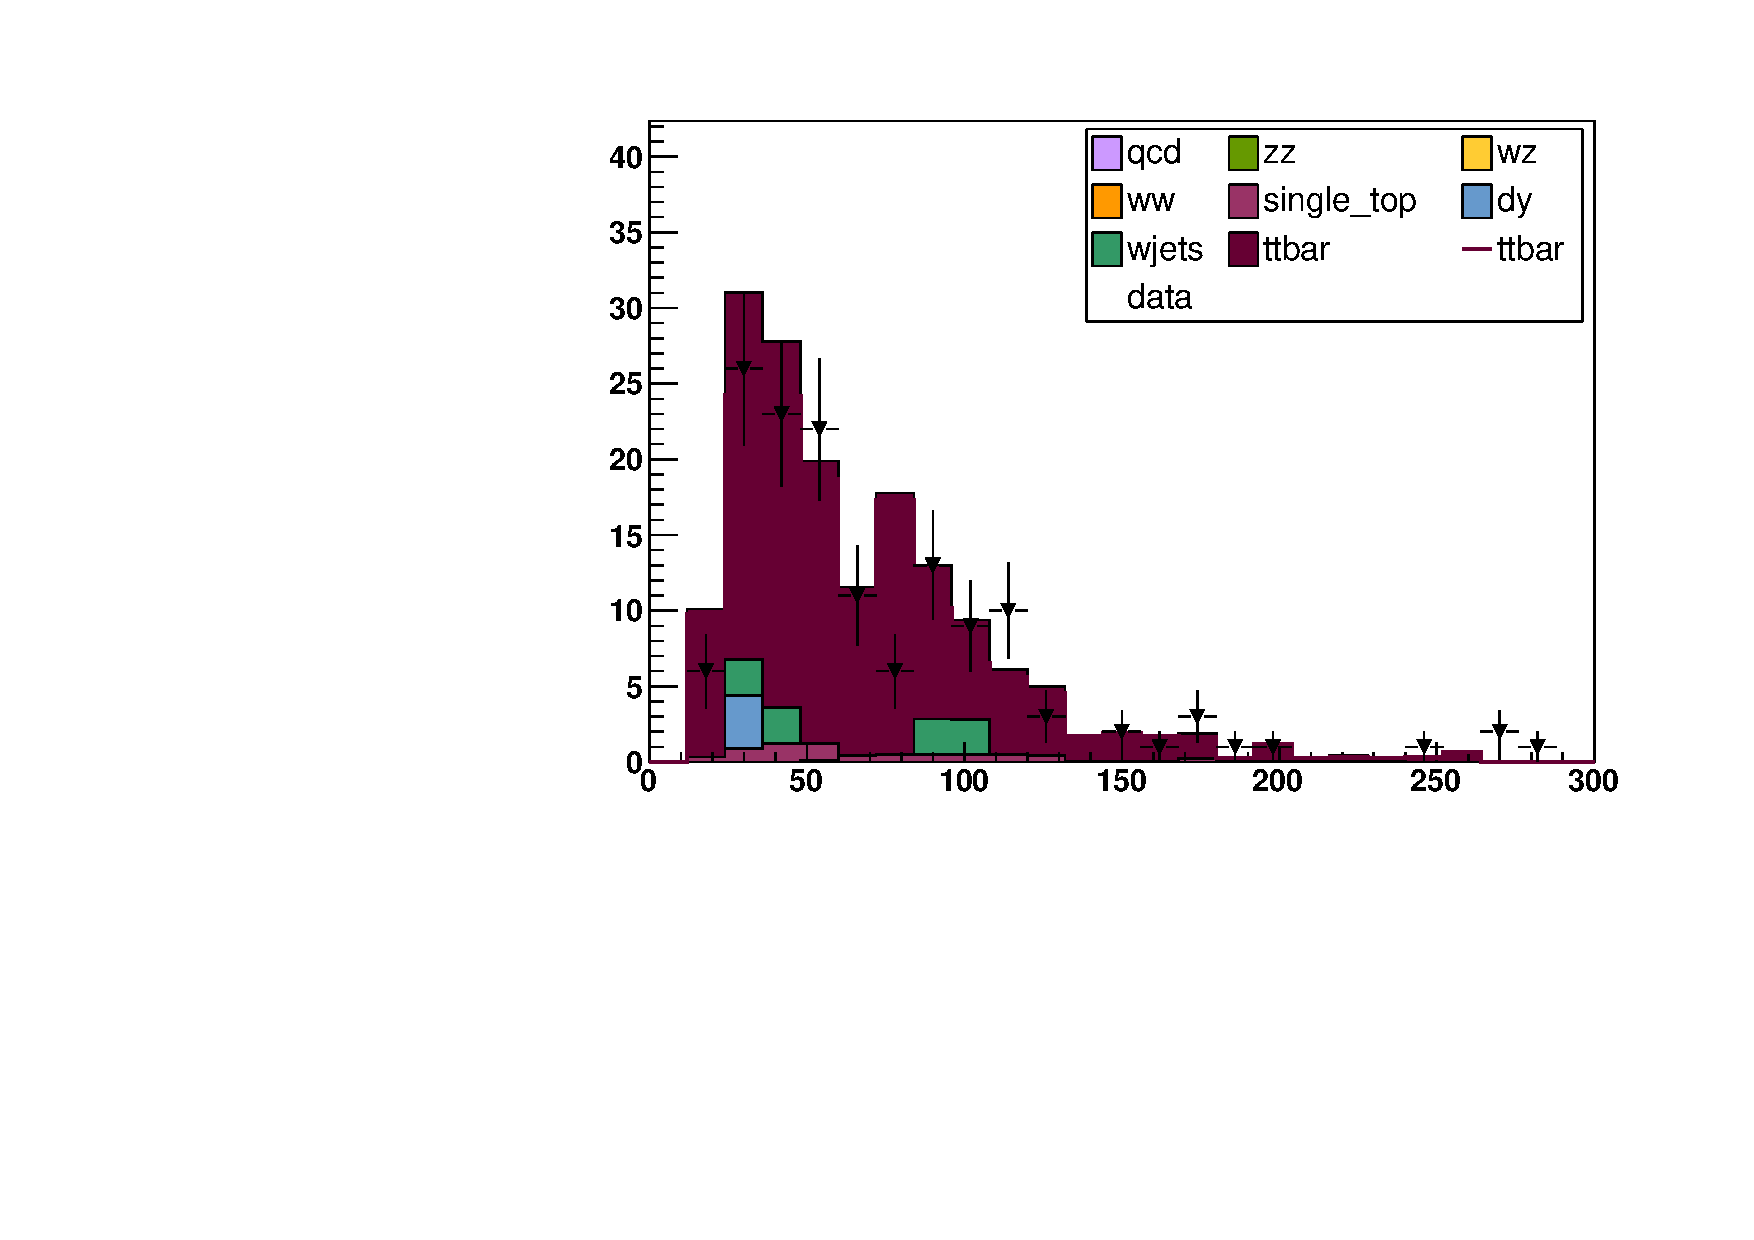
\includegraphics[scale=0.5]{fig/MET_Pt.pdf}};
			\node (B) at ($(A.south)!.00!(A.north)$) {Muon $p_T$ (GeV)};
		\end{tikzpicture}
	\end{center}
	\caption{The distribution of muon $p_T$ events passing the selection criteria}
	\label{fig:bgsubtraction}
\end{figure}
The resulting signal and background after the selection is shown in figure \ref{fig:bgsubtraction}.
The number of events is estimated as $N_\text{sig} / a \epsilon $, where $N_\text{sig}$ is the number of signal events passing the selection, $a$ is the acceptance and $\epsilon$ the trigger efficiency. Acceptance is estimated by applying our to MC data and taking the ratio of signal events before and after applying the cuts. Trigger efficiency is the ratio of of triggered and untriggered signal events while imposing the cuts. 

\subsection{Uncertainties}
Bins in histograms are assumed to be independently Poisson distributed. Therefore bins of height $N$ are assumed to have error $\sqrt{N}$, and the error of an integrated histogram is obtained through Gaussian error propagation from the bins to the integral. 
For acceptance, the error is given through propagation from error of the counted events passing the selection and the error of the total $t \overline{t}$ signal which is $\sqrt{7928.61}$. The error on the trigger efficiency also stems from Poisson-distributed bins.
\\ 
To obtain another estimation of the error for acceptance and trigger efficiency, one can also assume a binomial process. For the MC data this is applicable since there is a fixed number of trials, which can be assumed to pass with a certain probability. The number of successes in fixed amount of trials then follows a binomial distribution. For the trigger efficiency with $m$ out of $n$ events passing, one then obtains the binomial error estimate
\begin{equation}
	\sigma_\epsilon = \sqrt \frac{\epsilon(1-\epsilon)}{n}
\end{equation}
where $\epsilon = m/n$ is the expectation value. 
\\
In this report, the error was compared with the Poisson error and as a conservative estimate the larger error was used for further analysis (which was always the Poisson error). \\
To conclude, the statistical error of the resulting cross section is obtained from the error on events, acceptance and trigger efficiency.  
As the only source of systematic error, a $10\%$ relative error on luminosity is assumed. Since the cross section is multiplicative in the luminosity, it will have the same relative systematic error.

\subsection{Results}
The measured cross section is $\sigma = 173 \pm 21 (\text{stat}) \pm 17 (\text{sys}) \, \text{pb}$ which agrees well with the theory prediction \cite{topxs} of $\sigma_\text{pred} = 174 \pm 12$ pb. The number of observations and background events are $ N_\text{obs} = 141 \pm 12$ and $N_\text{bkg} = 50 \pm 5$ respectively. \\
The acceptance is $ a = 15.9 \pm  0.8 $\textperthousand \ (per mille), which results from $125 \pm 6$ out of $7929 \pm 89$ accepted MC signal events. The trigger efficiency is $\epsilon = 88.2 \pm 2.7 \%$ based on $126 \pm 6$ out of $142 \pm 6$ events passing the trigger criteria. 

\pagebreak
\section{W boson charge asymmetry}
\subsection{Introduction}
In this part, the $W$ boson charge asymmetry in the muonic channel of $W$ production is measured. The charge asymmetry $\mathcal{A}$ can be defined as 
\begin{equation}
	\mathcal{A} = \frac{N_+ - N_-}{N_+ + N_-}
\end{equation}
where $N_{+,-}$ are the number of events with a $\mu^{+,-}$ respectively. Since we expect a dependence from muon pseudorapidity $\eta$, we measure $\mathcal{A}(\eta)$ in different intervals of $\eta$. 
\subsection{Event selection and signal reconstruction}
The $W \rightarrow \mu \nu$ event candidates are selected by requiring at least one isolated muon with $p_T > 25$ GeV and relative isolation (as defined in the last section) $ < 0.1$. In addition, the muon pseudorapidity must fulfill $\eta < 2.0$. Furthermore, we ask for undetected neutrinos by requiring $\slashed{E}_T > 20$ GeV. This helps to suppress a lot of QCD and Drell-Yan background, since a large $\slashed{E}_T$ means that the neutrino comes from a primary vertex, and not from somewhere down the line. An overview of the events passing the selection is shown in figure \ref{fig:bkgsub2} where we show for $\mu^+$ and $\mu^-$ the pseudorapidity $\eta$ as well as the reconstructed $W$ mass.
\begin{figure}[!htb]
	\centering
	\begin{minipage}{.5\textwidth}
		\centering
		\begin{tikzpicture}
			\node[inner sep=0pt] (A) {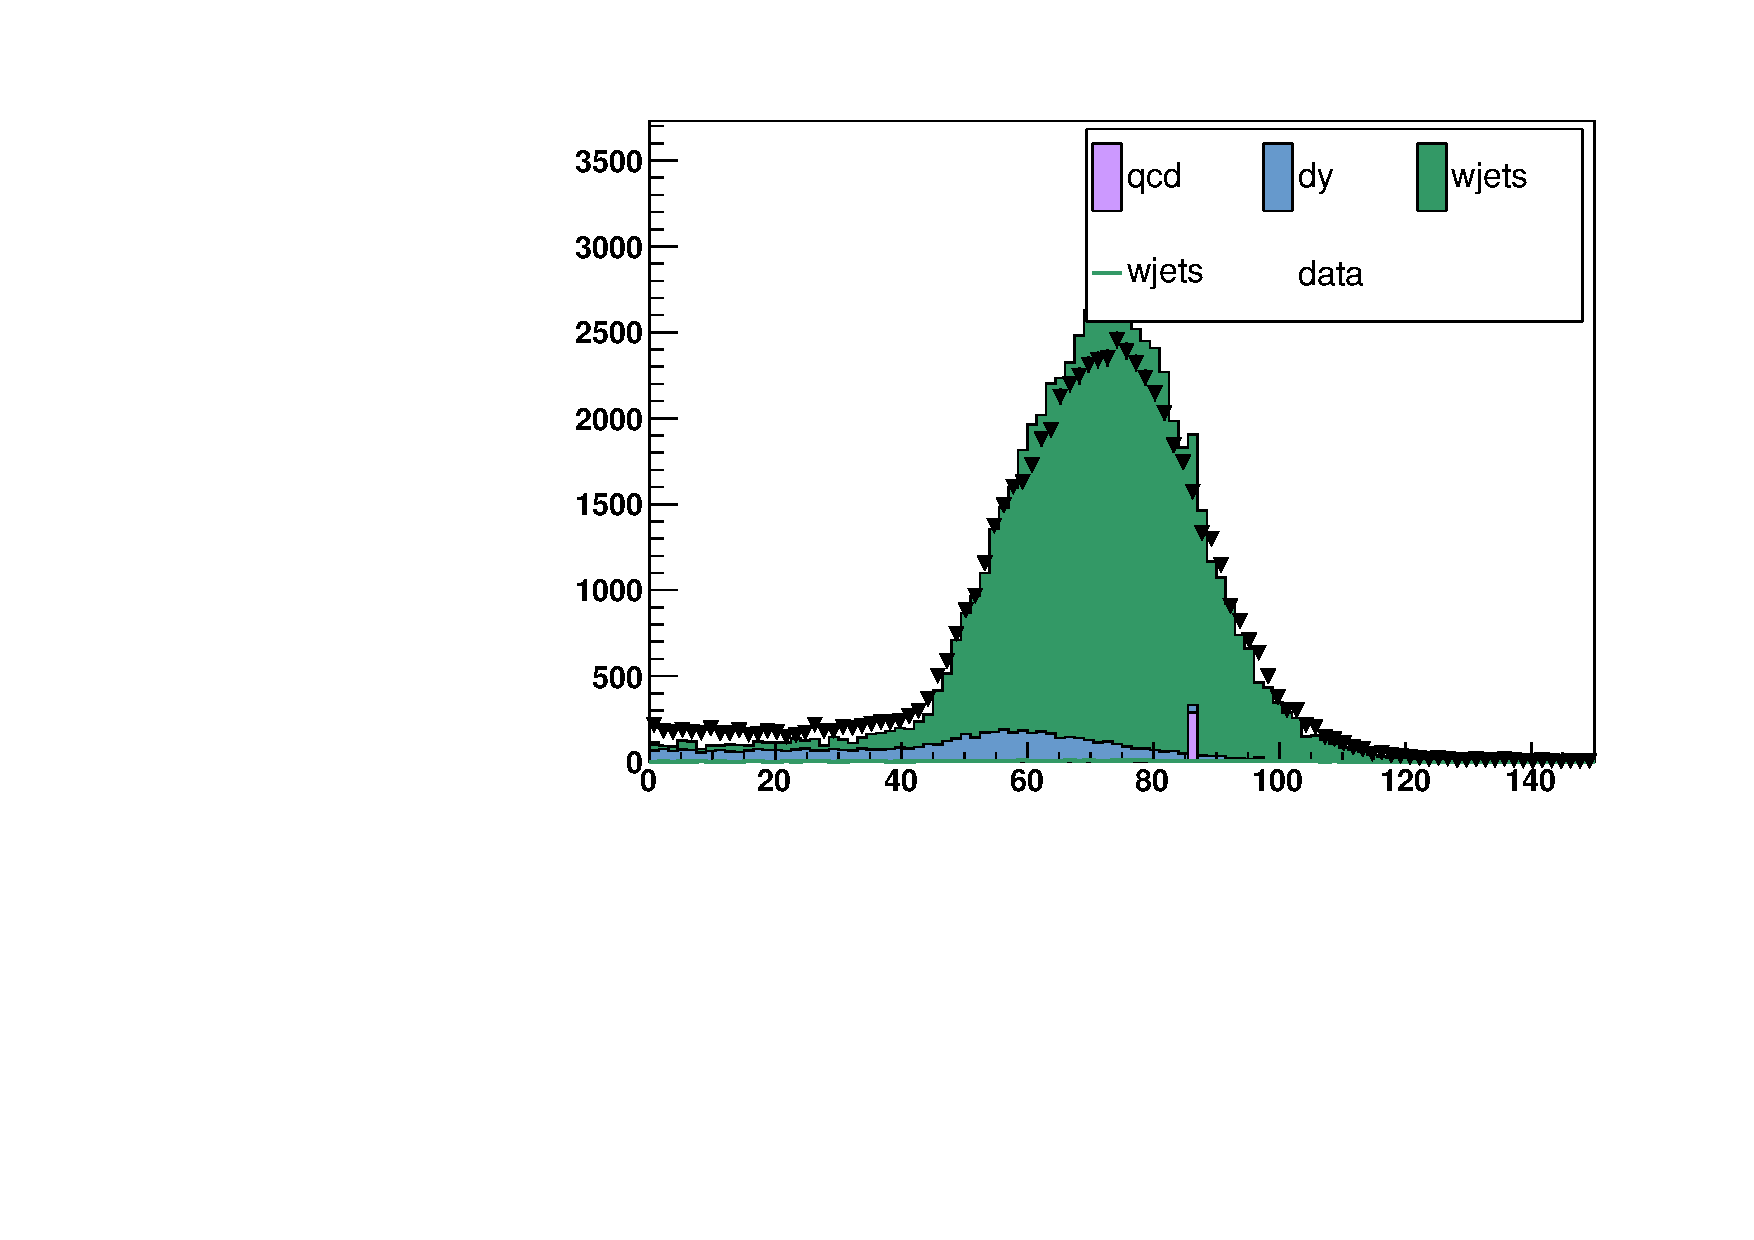
\includegraphics[width=1.0\linewidth]{fig/mWm.pdf}};
			\node (B) at ($(A.south)!.00!(A.north)$) {$m_W$ (GeV)};
		\end{tikzpicture}
	\end{minipage}%
	\begin{minipage}{.5\textwidth}
		\centering
		\begin{tikzpicture}
			\node[inner sep=0pt] (A) {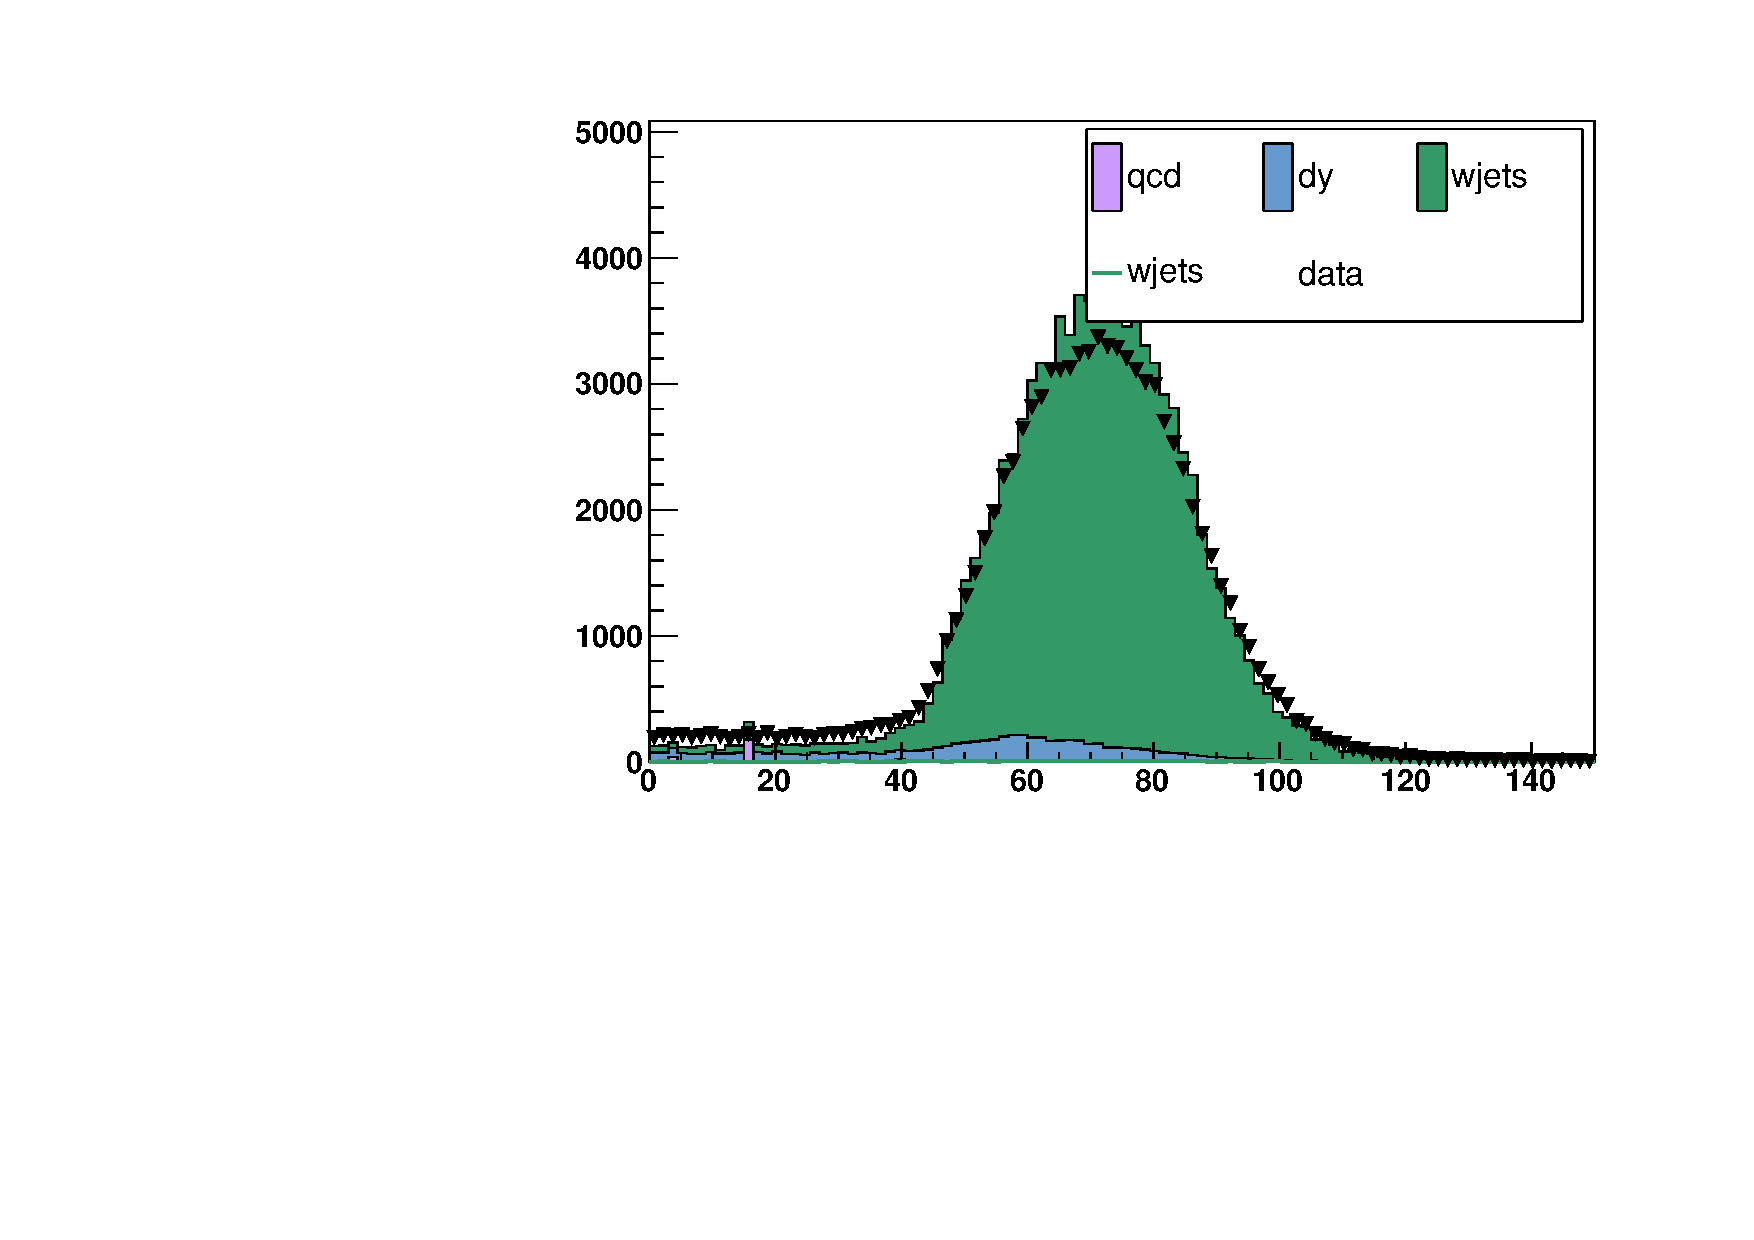
\includegraphics[width=1.0\linewidth]{fig/mWp.pdf}};
			\node (B) at ($(A.south)!.00!(A.north)$) {$m_W$ (GeV)};
		\end{tikzpicture}
	\end{minipage}
	\begin{minipage}{.5\textwidth}
		\centering
		\begin{tikzpicture}
			\node[inner sep=0pt] (A) {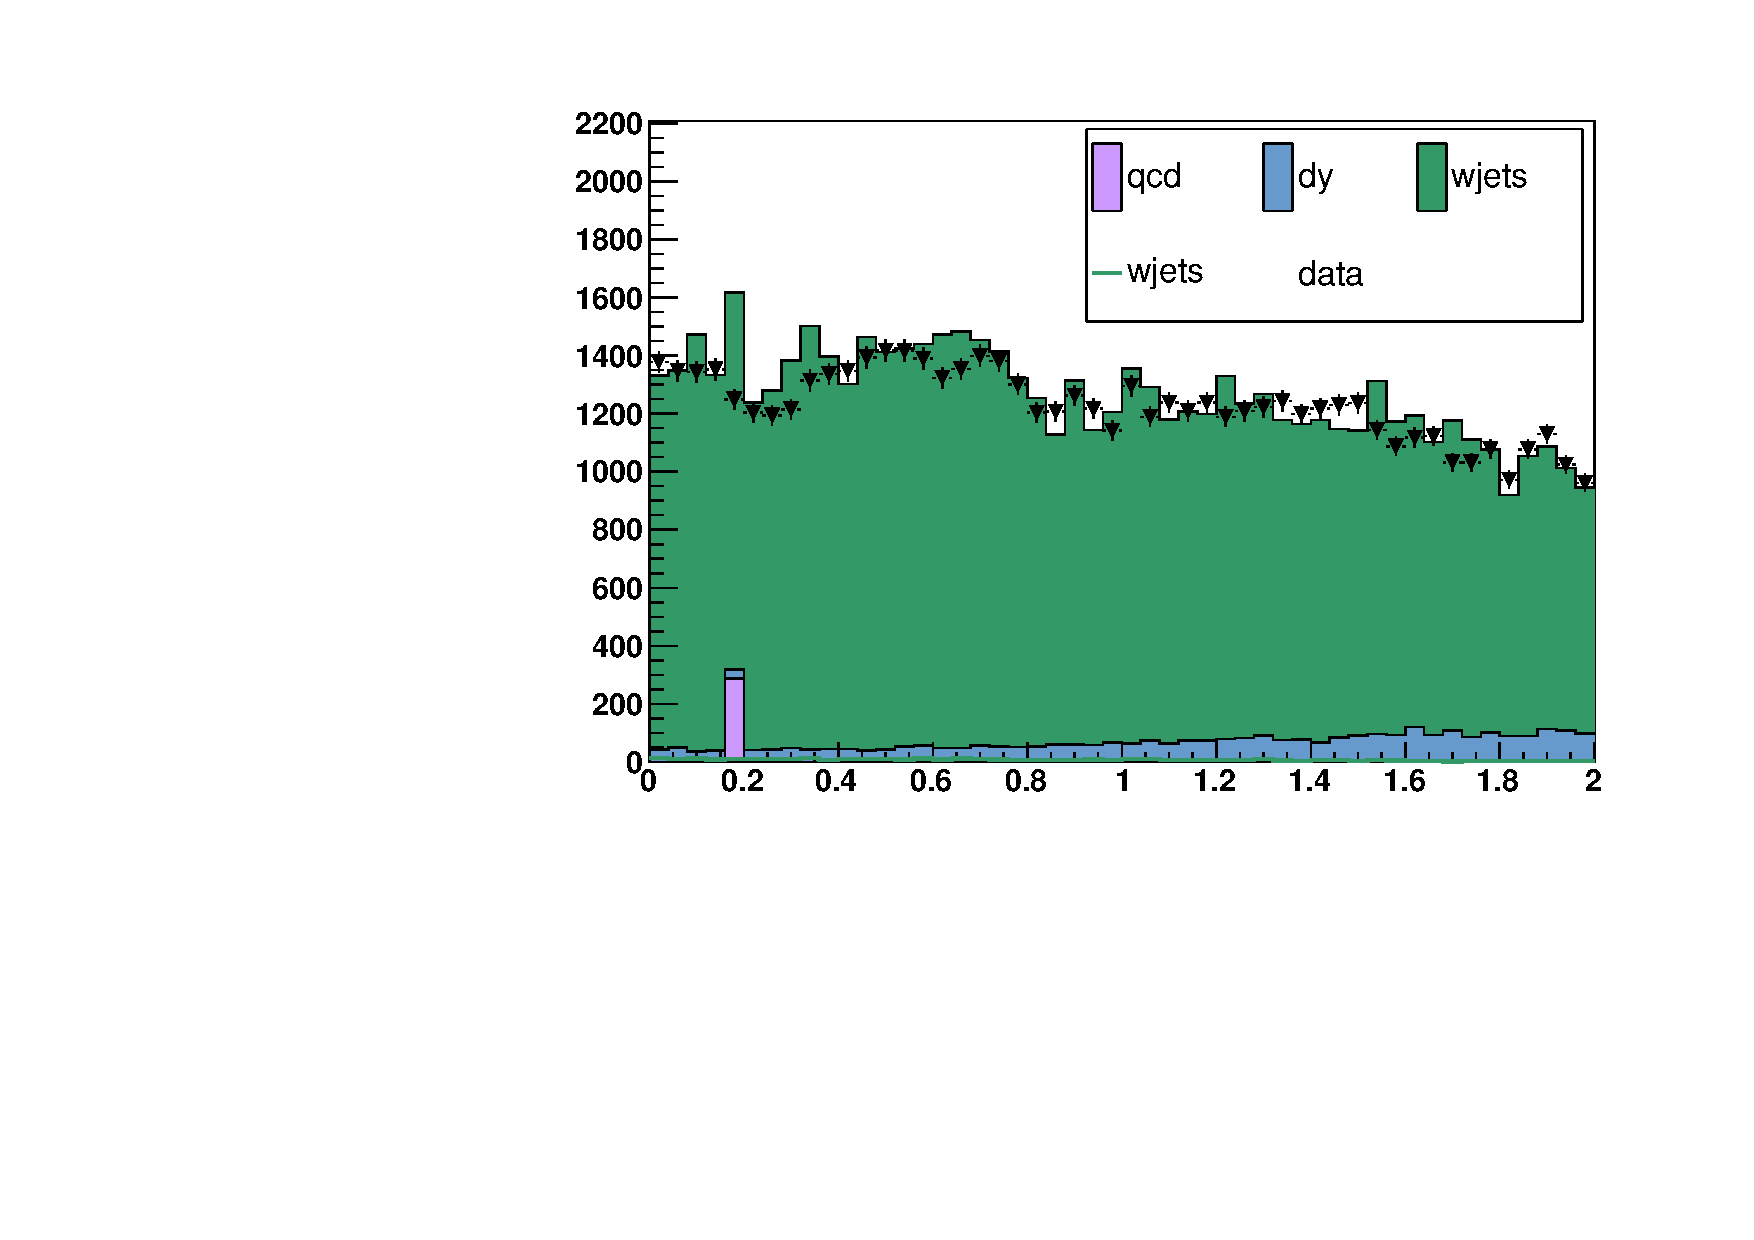
\includegraphics[width=1.0\linewidth]{fig/Muonm_eta.pdf}};
			\node (B) at ($(A.south)!.00!(A.north)$) {Muon $\eta$};
		\end{tikzpicture}
	\end{minipage}%
	\begin{minipage}{.5\textwidth}
		\centering
		\begin{tikzpicture}
			\node[inner sep=0pt] (A) {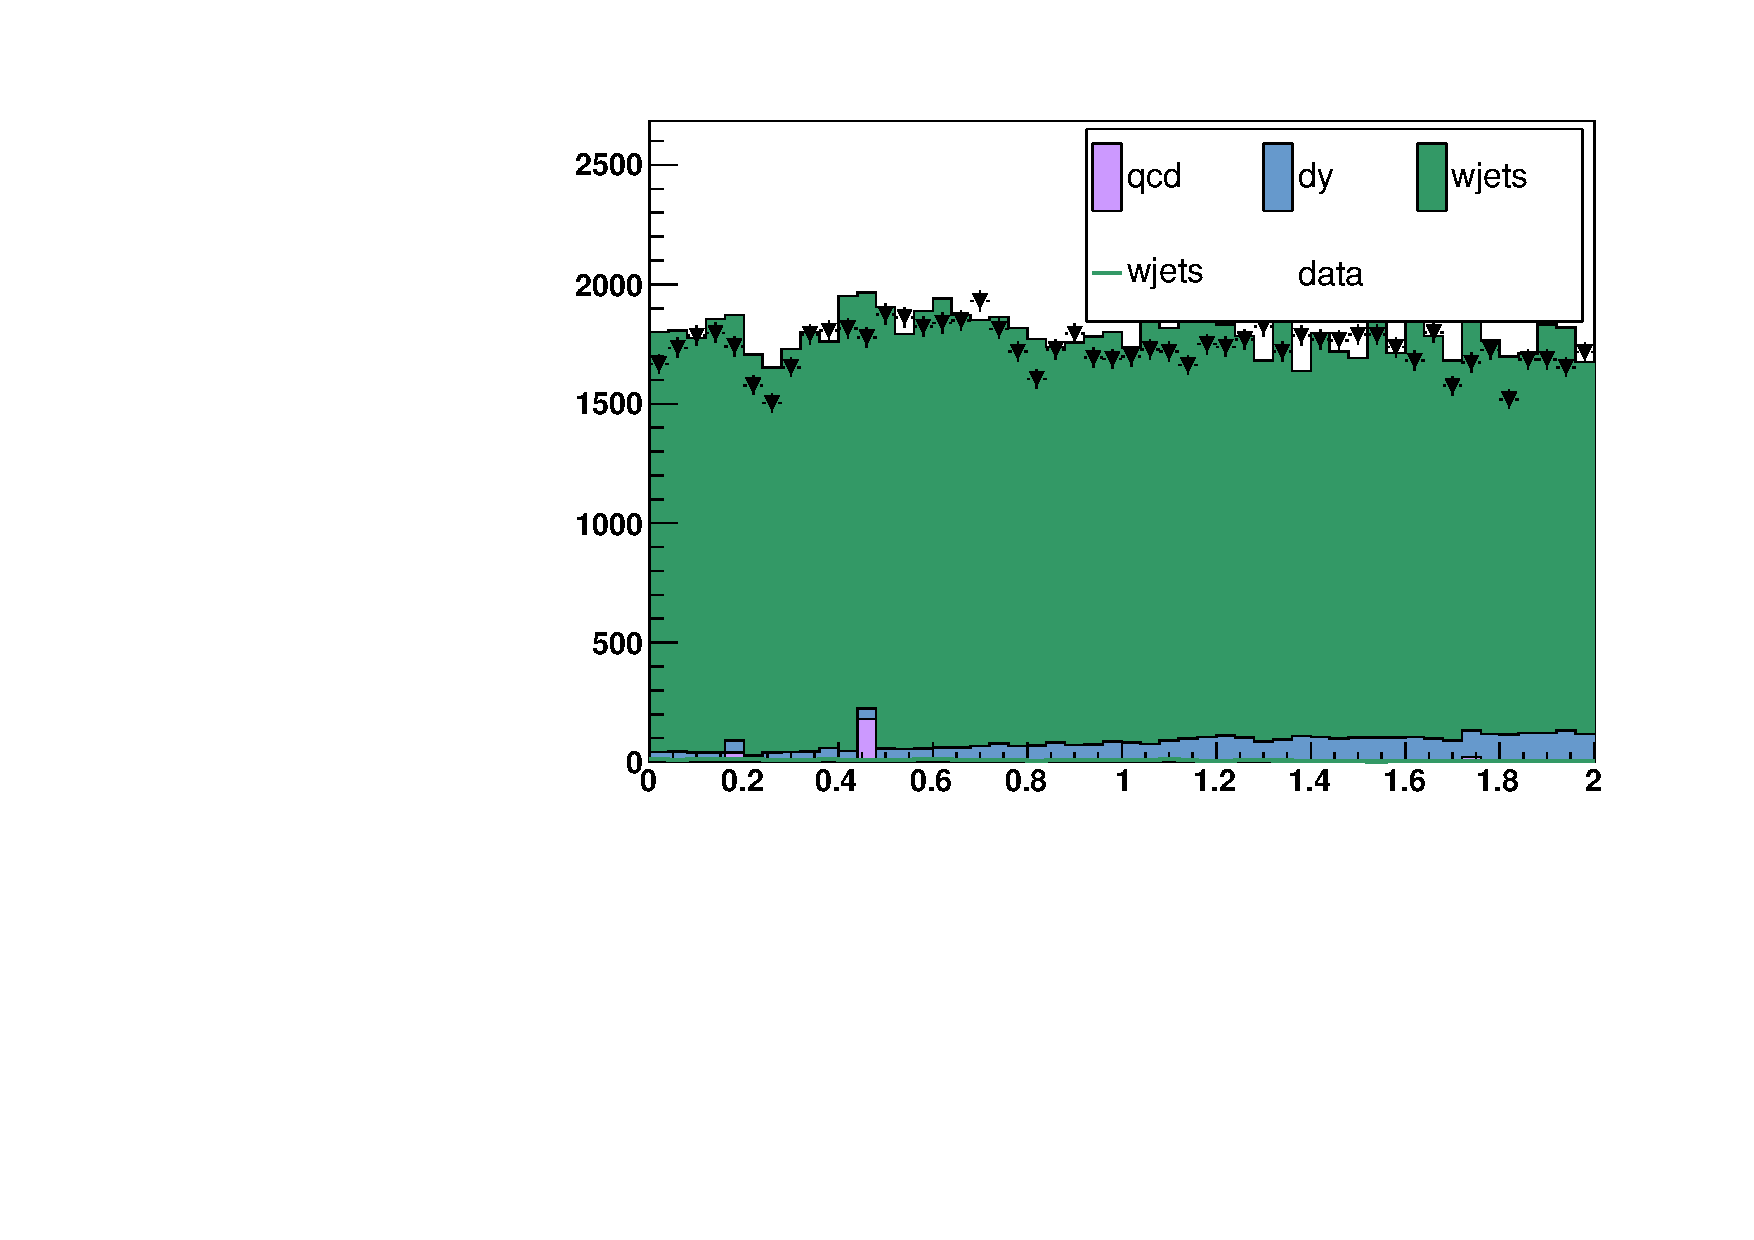
\includegraphics[width=1.0\linewidth]{fig/Muonp_eta.pdf}};
			\node (B) at ($(A.south)!.00!(A.north)$) {Muon $\eta$};
		\end{tikzpicture}
	\end{minipage}
	\caption{The distribution events passing the selection criteria for $\mu^-$ (left) and $\mu^+$ (right). Top: The distribution of the reconstructed $W$ mass $m_W$. Bottom: The distribution of muon pseudorapidity $\eta$.}
	\label{fig:bkgsub2}
\end{figure}
The latter is reconstructed as  
\begin{equation}
	m_W ^2 = (p_{\mu,T} + \slashed{p}_{T})^2
\end{equation}
where $p_{\mu,T}$ is the transverse muon four-momentum and $ \slashed{p}_{T}$ the transverse missing four-momentum.
\\
In each bin, we account for acceptance and trigger efficiency separately. The estimation of the uncertainties for number of events, acceptances and trigger efficiencies follows the same procedure outlined in the last section. 

\subsection{Results}	
The measured $\mathcal{A}(\eta)$ is summarized in figure \ref{fig:asymm}. Since many raw numbers are used for the result, we don't list them here. The error of $\mathcal{A}(\eta)$ is obtained through Gaussian propagation by assuming independence of $N_-$ and $N_+$. 
\begin{figure}[!htb]
	\begin{center}
	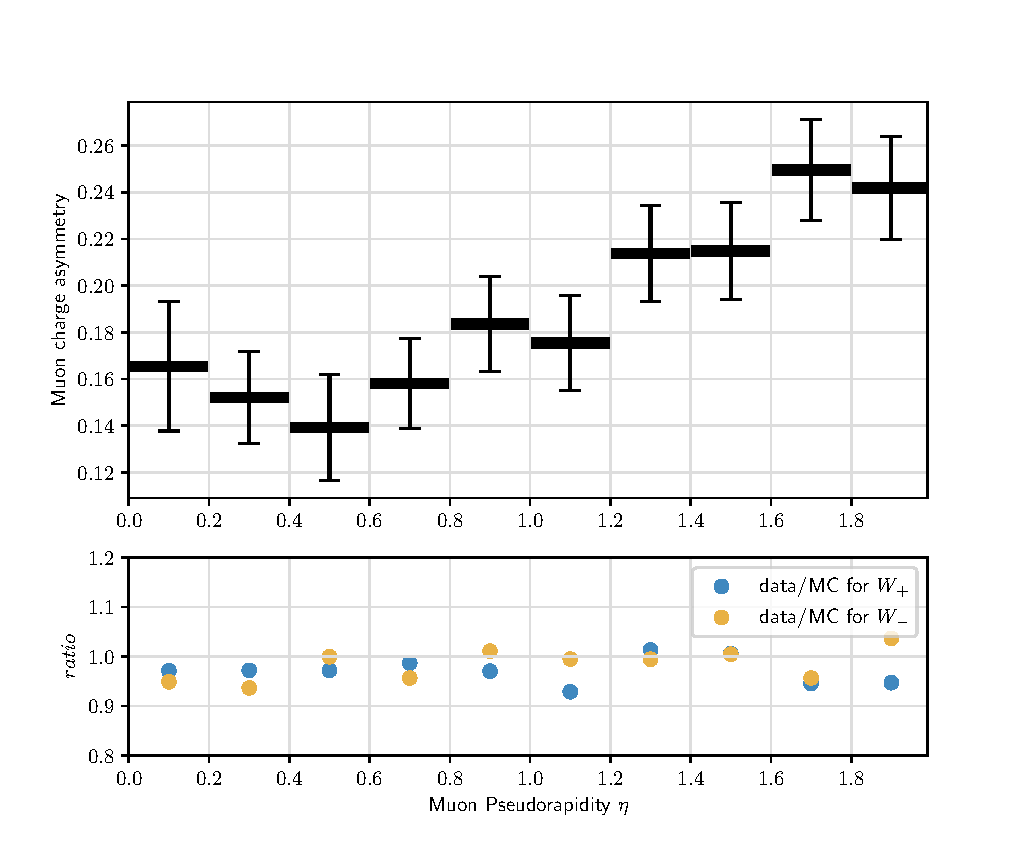
\includegraphics[scale=0.7]{fig/asymmetry.pdf}
	\end{center}
	\caption{Top: The $W$ boson charge asymmetry $\mathcal{A}(\eta)$ measured in different intervals of $\eta$. Bottom: The ratio of data and MC events for $W^+$ and $W^-$ separately. }
	\label{fig:asymm}
\end{figure}
It can be observed that the asymmetry is approximately $15 \pm 3$ \% at small values of $\eta$ and increases towards approximately $24 \pm 2$ \% for $1.8 < \eta < 2.0$. Due to the large quantity of raw values used to compute the results, we do not list them here, instead we refer to the code used for the analysis which can be found in the project's github repository (see section 1).
\subsection{Discussion and Outlook}
As it can be observed in figure \ref{fig:asymm}, the agreement between the data and MC events can be considered sufficient for the asymmetry error targeted in this report. To make the comparison more precise, the $\xi^2/DoF$ was computed in each bin, where a maximum value of $\xi^2/DoF = 3.8$ was observed. Nevertheless, there is some discrepancy, for example in the region $1.0 < \eta < 1.2$ for $W_+$. As for the reason of the discrepancy, it can be speculated that it results most likely from the finite order approximation of the monte carlo data. It should then decrease if one uses a more accurate event generator for the MC data (e.g. one that goes to higher order in perturbation theory).  
\\
To deal with this, it would be advantageous to perform a maximum-likelihood fit to separate signal from background with some model. However, the fit should not be performed in the $\eta$ distribution since both signal and background seem to be more or less linear in that variable. In the $\eta$ distribution it would therefore be close to impossible to separate signal from background. Instead, one could for example use the reconstructed $W$ mass from the top row of fig \ref{fig:bkgsub2}, where it might be possible to use a Gaussian model for the signal, and perhaps an error function plus Gaussian for the background. One could then compare the two measurements. 
\bibliography{bibliography.bib}
\bibliographystyle{JHEP}

\end{document}



















